\documentclass[border=1pt]{standalone}
\usepackage[dvipsnames]{xcolor}
\usepackage{amssymb}
\usepackage{tikz}                       % Graphen und kommutative Diagramme
\usetikzlibrary{patterns}               % Um schraffierte Formen in der tikzpicture-Umgebung zu zeichnen.
\usetikzlibrary{shapes}                 % Vielecke

\begin{document}

\newcommand{\ul}{\underline}
\newcommand{\A}{\mathbb A}

\newcommand{\radmult}
{
    \ensuremath{
	\tikz[baseline={([yshift=-1pt]current bounding box.center)}, x=5pt, y=2.5pt, every node/.style={shape=circle, fill=black, inner sep=.8pt}]{
	    \draw[line width=0.9pt] (5, 0) -- (3, 0);
	    \draw[line width=0.9pt] (2, 0) -- (0, 0);
	    \filldraw (3, 0) circle (1pt);
	    \filldraw (2, 0) circle (1pt);
	}
    }
}

\newcommand{\equals}
{
    \ensuremath{
	\tikz[baseline={([yshift=2pt]current bounding box.center)}, x=5pt, y=2.5pt]{
	    \node (0, 0) {$=$};
	}
    }
}

\centering
\begin{minipage}{.3\textwidth}
\centering
\resizebox{!}{3cm}{
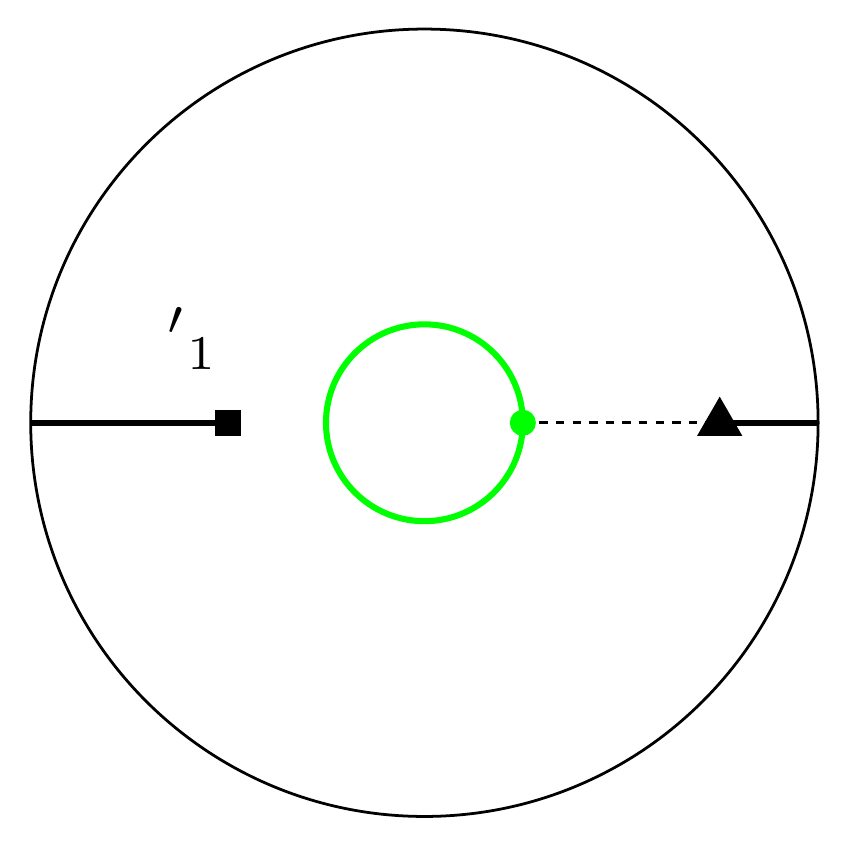
\begin{tikzpicture}[x=1.25cm, y=1.25cm, line width=1pt]
    % draw inner and outer circles
    \draw[color=green, line width = 2.2pt] (0, 0) circle (1);
    \draw[color=black] (0, 0) circle (4);
    
    % draw 0 line
    \draw[color=black, dashed] (0 : 1) -- (0 : 4); 
    
    % draw slits
    \draw[color=black, line width=2.2pt] (0 : 3) -- (0 : 4);
    \node[color = black, fill = black, regular polygon, regular polygon sides = 3] at (0 : 3){};

    \draw[color=black, line width=2.2pt] (180 : 2) -- (180 : 4);
    \node[color=black, fill=black, regular polygon, regular polygon sides = 4] at (180 : 2) {};

    % draw symbols
    \node[scale = 2.5, fill = white] at (160 : 2.5) {${\A'}_1$};

    % draw marked point
    \node[fill = green, circle] at (0 : 1) {};
    
    \end{tikzpicture}
}
\end{minipage}
\centering
\begin{minipage}{.3\textwidth}
\centering
\resizebox{!}{3cm}{
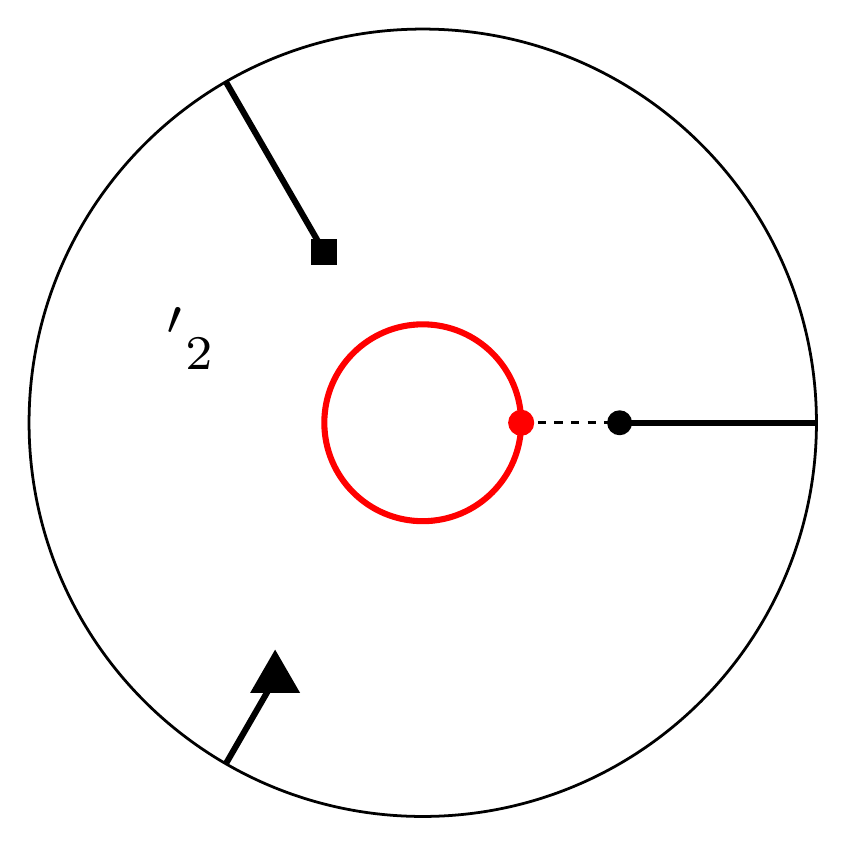
\begin{tikzpicture}[x=1.25cm, y=1.25cm, line width=1pt]
    % draw inner and outer circles
    \draw[color=red, line width = 2.2pt] (0, 0) circle (1);
    \draw[color=black] (0, 0) circle (4);
    
    % draw 0 line
    \draw[color=black, dashed] (0 : 1) -- (0 : 4); 
    
    % draw slits
    \draw[color=black, line width=2.2pt] (0 : 2) -- (0 : 4);
    \filldraw[color = black, fill = black] (0 : 2) circle (4pt);

    \draw[color=black, line width=2.2pt] (120 : 2) -- (120 : 4);
    \node[color=black, fill=black, regular polygon, regular polygon sides = 4] at (120 : 2) {};
    
    \draw[color=black, line width=2.2pt] (240: 3) -- (240 : 4);
    \node[draw = black, fill = black, regular polygon, regular polygon sides = 3] at (240 : 3){};

    % draw symbols
    \node[scale = 2.5, fill = white] at (160 : 2.5) {${\A'}_2$};
 
    % draw marked point
    \node[fill = red, circle] at (0 : 1) {};
    
    \end{tikzpicture}
}
\end{minipage}

\centering
\begin{minipage}{.3\textwidth}
\centering
\resizebox{!}{3cm}{
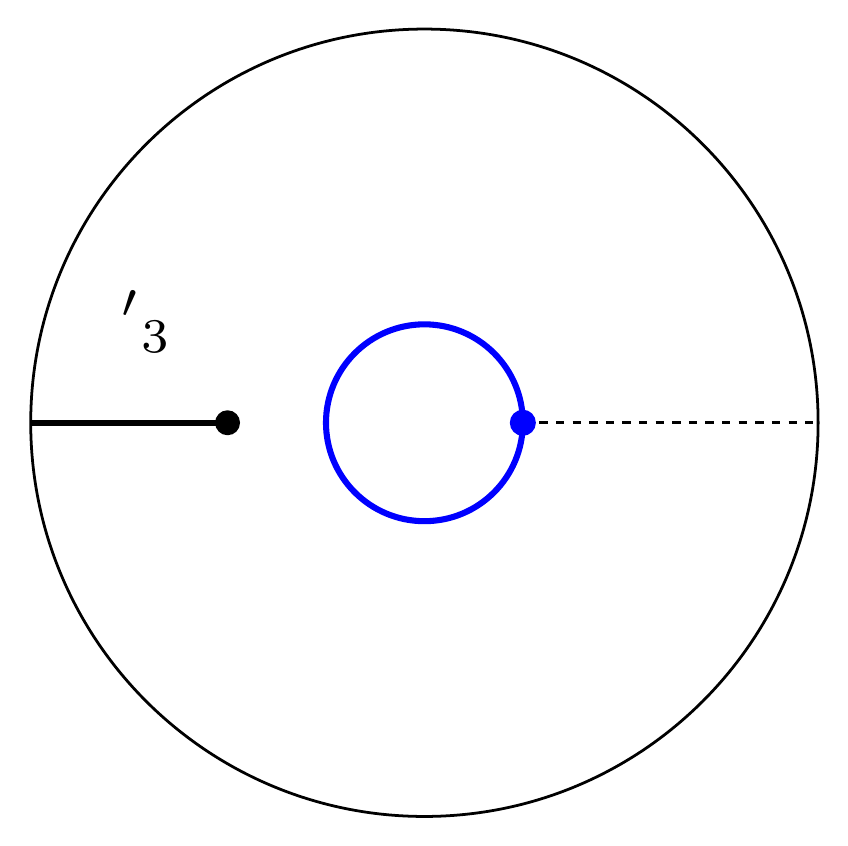
\begin{tikzpicture}[x=1.25cm, y=1.25cm, line width=1pt]
    % draw inner and outer circles
    \draw[color=blue, line width = 2.2pt] (0, 0) circle (1);
    \draw[color=black] (0, 0) circle (4);
    
    % draw 0 line
    \draw[color=black, dashed] (0 : 1) -- (0 : 4); 
    
    % draw slits
    \draw[color=black, line width=2.2pt] (180 : 2) -- (180 : 4);
    \filldraw[color = black, fill = black] (180 : 2) circle (4pt);
    
    % draw symbols
    \node[scale = 2.5, fill = white] at (160 : 3) {${\A'}_3$};
    
    % draw marked point
    \node[fill = blue, circle] at (0 : 1) {};
    
    \end{tikzpicture}
}
\end{minipage}

\end{document}